\documentclass[a4paper]{book}
\usepackage{makeidx}
\usepackage{natbib}
\usepackage{graphicx}
\usepackage{multicol}
\usepackage{float}
\usepackage{listings}
\usepackage{color}
\usepackage{ifthen}
\usepackage[table]{xcolor}
\usepackage{textcomp}
\usepackage{alltt}
\usepackage{ifpdf}
\ifpdf
\usepackage[pdftex,
            pagebackref=true,
            colorlinks=true,
            linkcolor=blue,
            unicode
           ]{hyperref}
\else
\usepackage[ps2pdf,
            pagebackref=true,
            colorlinks=true,
            linkcolor=blue,
            unicode
           ]{hyperref}
\usepackage{pspicture}
\fi
\usepackage[utf8]{inputenc}
\usepackage{mathptmx}
\usepackage[scaled=.90]{helvet}
\usepackage{courier}
\usepackage{sectsty}
\usepackage[titles]{tocloft}
\usepackage{doxygen}
\lstset{language=C++,inputencoding=utf8,basicstyle=\footnotesize,breaklines=true,breakatwhitespace=true,tabsize=8,numbers=left }
\makeindex
\setcounter{tocdepth}{3}
\renewcommand{\footrulewidth}{0.4pt}
\renewcommand{\familydefault}{\sfdefault}
\hfuzz=15pt
\setlength{\emergencystretch}{15pt}
\hbadness=750
\tolerance=750
\begin{document}
\hypersetup{pageanchor=false,citecolor=blue}
\begin{titlepage}
\vspace*{7cm}
\begin{center}
{\Large \-Programowanieobiektowe \\[1ex]\large v1 }\\
\vspace*{1cm}
{\large \-Generated by Doxygen 1.7.6.1}\\
\vspace*{0.5cm}
{\small Wed Nov 14 2012 19:15:14}\\
\end{center}
\end{titlepage}
\clearemptydoublepage
\pagenumbering{roman}
\tableofcontents
\clearemptydoublepage
\pagenumbering{arabic}
\hypersetup{pageanchor=true,citecolor=blue}
\chapter{\-Namespace \-Index}
\section{\-Namespace \-List}
\-Here is a list of all namespaces with brief descriptions\-:\begin{DoxyCompactList}
\item\contentsline{section}{\hyperlink{namespaceOOP}{\-O\-O\-P} }{\pageref{namespaceOOP}}{}
\end{DoxyCompactList}

\chapter{\-Class \-Index}
\section{\-Class \-List}
\-Here are the classes, structs, unions and interfaces with brief descriptions\-:\begin{DoxyCompactList}
\item\contentsline{section}{\hyperlink{classVector}{\-Vector} }{\pageref{classVector}}{}
\end{DoxyCompactList}

\chapter{\-File \-Index}
\section{\-File \-List}
\-Here is a list of all files with brief descriptions\-:\begin{DoxyCompactList}
\item\contentsline{section}{\hyperlink{lab4b__main_8cpp}{lab4b\-\_\-main.\-cpp} }{\pageref{lab4b__main_8cpp}}{}
\item\contentsline{section}{\hyperlink{Vector_8cpp}{\-Vector.\-cpp} }{\pageref{Vector_8cpp}}{}
\item\contentsline{section}{\hyperlink{Vector_8h}{\-Vector.\-h} }{\pageref{Vector_8h}}{}
\end{DoxyCompactList}

\chapter{\-Namespace \-Documentation}
\hypertarget{namespaceOOP}{\section{\-O\-O\-P \-Namespace \-Reference}
\label{namespaceOOP}\index{\-O\-O\-P@{\-O\-O\-P}}
}
\subsection*{\-Classes}
\begin{DoxyCompactItemize}
\item 
class \hyperlink{classOOP_1_1array}{array}
\item 
class \hyperlink{classOOP_1_1BaseClass}{\-Base\-Class}
\item 
class \hyperlink{classOOP_1_1CountedPtr}{\-Counted\-Ptr}
\end{DoxyCompactItemize}
\subsection*{\-Typedefs}
\begin{DoxyCompactItemize}
\item 
typedef \hyperlink{classOOP_1_1BaseClass}{\-Base\-Class} \hyperlink{namespaceOOP_a98bf9fa44d8f36499284c9d57c1958aa}{value\-\_\-type}
\end{DoxyCompactItemize}
\subsection*{\-Functions}
\begin{DoxyCompactItemize}
\item 
void \hyperlink{namespaceOOP_a32e75bb4328dbb5e86e98a8af0a5cf61}{print\-\_\-tab\-\_\-el} (const \hyperlink{classOOP_1_1array}{array} \&tab2)
\item 
ostream \& \hyperlink{namespaceOOP_a3f50dd68985954d3519768fe0da14797}{operator$<$$<$} (ostream \&stream, \hyperlink{classOOP_1_1BaseClass}{\-Base\-Class} \&base)
\end{DoxyCompactItemize}


\subsection{\-Typedef \-Documentation}
\hypertarget{namespaceOOP_a98bf9fa44d8f36499284c9d57c1958aa}{\index{\-O\-O\-P@{\-O\-O\-P}!value\-\_\-type@{value\-\_\-type}}
\index{value\-\_\-type@{value\-\_\-type}!OOP@{\-O\-O\-P}}
\subsubsection[{value\-\_\-type}]{\setlength{\rightskip}{0pt plus 5cm}typedef {\bf \-Base\-Class} {\bf \-O\-O\-P\-::value\-\_\-type}}}\label{namespaceOOP_a98bf9fa44d8f36499284c9d57c1958aa}


\subsection{\-Function \-Documentation}
\hypertarget{namespaceOOP_a3f50dd68985954d3519768fe0da14797}{\index{\-O\-O\-P@{\-O\-O\-P}!operator$<$$<$@{operator$<$$<$}}
\index{operator$<$$<$@{operator$<$$<$}!OOP@{\-O\-O\-P}}
\subsubsection[{operator$<$$<$}]{\setlength{\rightskip}{0pt plus 5cm}ostream\& \-O\-O\-P\-::operator$<$$<$ (
\begin{DoxyParamCaption}
\item[{ostream \&}]{stream, }
\item[{\-Base\-Class \&}]{base}
\end{DoxyParamCaption}
)}}\label{namespaceOOP_a3f50dd68985954d3519768fe0da14797}
\hypertarget{namespaceOOP_a32e75bb4328dbb5e86e98a8af0a5cf61}{\index{\-O\-O\-P@{\-O\-O\-P}!print\-\_\-tab\-\_\-el@{print\-\_\-tab\-\_\-el}}
\index{print\-\_\-tab\-\_\-el@{print\-\_\-tab\-\_\-el}!OOP@{\-O\-O\-P}}
\subsubsection[{print\-\_\-tab\-\_\-el}]{\setlength{\rightskip}{0pt plus 5cm}void {\bf \-O\-O\-P\-::print\-\_\-tab\-\_\-el} (
\begin{DoxyParamCaption}
\item[{const array \&}]{tab2}
\end{DoxyParamCaption}
)}}\label{namespaceOOP_a32e75bb4328dbb5e86e98a8af0a5cf61}

\chapter{\-Class \-Documentation}
\hypertarget{classOOP_1_1array}{\section{\-O\-O\-P\-:\-:array \-Class \-Reference}
\label{classOOP_1_1array}\index{\-O\-O\-P\-::array@{\-O\-O\-P\-::array}}
}


{\ttfamily \#include $<$array.\-h$>$}



\-Collaboration diagram for \-O\-O\-P\-:\-:array\-:
\nopagebreak
\begin{figure}[H]
\begin{center}
\leavevmode
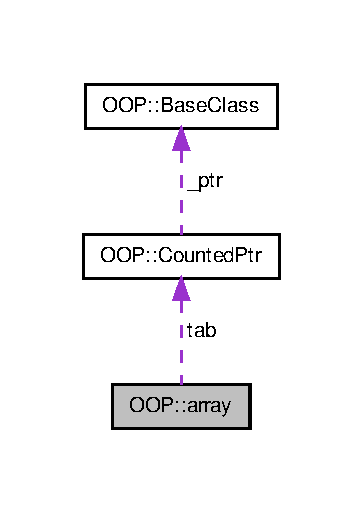
\includegraphics[width=174pt]{classOOP_1_1array__coll__graph}
\end{center}
\end{figure}
\subsection*{\-Public \-Member \-Functions}
\begin{DoxyCompactItemize}
\item 
\hyperlink{classOOP_1_1array_a387217686b62bffe5f8aac23569573cb}{array} ()
\item 
void \hyperlink{classOOP_1_1array_aacf55ebc981f43f79f14b6346f9a3104}{push\-\_\-back} (\hyperlink{classOOP_1_1BaseClass}{\-Base\-Class} $\ast$element)
\end{DoxyCompactItemize}
\subsection*{\-Private \-Member \-Functions}
\begin{DoxyCompactItemize}
\item 
void \hyperlink{classOOP_1_1array_ab525b43e208a38c090331d59fc19f72c}{rozszerz} ()
\end{DoxyCompactItemize}
\subsection*{\-Private \-Attributes}
\begin{DoxyCompactItemize}
\item 
\hyperlink{classOOP_1_1CountedPtr}{\-Counted\-Ptr} $\ast$ \hyperlink{classOOP_1_1array_aad69708fa28a7012340355dcb8866ae3}{tab}
\item 
int \hyperlink{classOOP_1_1array_a22f31b91340f38f9acd0ed21814fff86}{ilosc}
\end{DoxyCompactItemize}
\subsection*{\-Friends}
\begin{DoxyCompactItemize}
\item 
void \hyperlink{classOOP_1_1array_a8a63fdc403051bf98b236855584dbe57}{print\-\_\-tab\-\_\-el} (const \hyperlink{classOOP_1_1array}{array} \&tab2)
\end{DoxyCompactItemize}


\subsection{\-Constructor \& \-Destructor \-Documentation}
\hypertarget{classOOP_1_1array_a387217686b62bffe5f8aac23569573cb}{\index{\-O\-O\-P\-::array@{\-O\-O\-P\-::array}!array@{array}}
\index{array@{array}!OOP::array@{\-O\-O\-P\-::array}}
\subsubsection[{array}]{\setlength{\rightskip}{0pt plus 5cm}{\bf \-O\-O\-P\-::array\-::array} (
\begin{DoxyParamCaption}
{}
\end{DoxyParamCaption}
)}}\label{classOOP_1_1array_a387217686b62bffe5f8aac23569573cb}


\subsection{\-Member \-Function \-Documentation}
\hypertarget{classOOP_1_1array_aacf55ebc981f43f79f14b6346f9a3104}{\index{\-O\-O\-P\-::array@{\-O\-O\-P\-::array}!push\-\_\-back@{push\-\_\-back}}
\index{push\-\_\-back@{push\-\_\-back}!OOP::array@{\-O\-O\-P\-::array}}
\subsubsection[{push\-\_\-back}]{\setlength{\rightskip}{0pt plus 5cm}void {\bf \-O\-O\-P\-::array\-::push\-\_\-back} (
\begin{DoxyParamCaption}
\item[{{\bf \-Base\-Class} $\ast$}]{element}
\end{DoxyParamCaption}
)}}\label{classOOP_1_1array_aacf55ebc981f43f79f14b6346f9a3104}
\hypertarget{classOOP_1_1array_ab525b43e208a38c090331d59fc19f72c}{\index{\-O\-O\-P\-::array@{\-O\-O\-P\-::array}!rozszerz@{rozszerz}}
\index{rozszerz@{rozszerz}!OOP::array@{\-O\-O\-P\-::array}}
\subsubsection[{rozszerz}]{\setlength{\rightskip}{0pt plus 5cm}void {\bf \-O\-O\-P\-::array\-::rozszerz} (
\begin{DoxyParamCaption}
{}
\end{DoxyParamCaption}
)\hspace{0.3cm}{\ttfamily  \mbox{[}private\mbox{]}}}}\label{classOOP_1_1array_ab525b43e208a38c090331d59fc19f72c}


\subsection{\-Friends \-And \-Related \-Function \-Documentation}
\hypertarget{classOOP_1_1array_a8a63fdc403051bf98b236855584dbe57}{\index{\-O\-O\-P\-::array@{\-O\-O\-P\-::array}!print\-\_\-tab\-\_\-el@{print\-\_\-tab\-\_\-el}}
\index{print\-\_\-tab\-\_\-el@{print\-\_\-tab\-\_\-el}!OOP::array@{\-O\-O\-P\-::array}}
\subsubsection[{print\-\_\-tab\-\_\-el}]{\setlength{\rightskip}{0pt plus 5cm}void {\bf print\-\_\-tab\-\_\-el} (
\begin{DoxyParamCaption}
\item[{const {\bf array} \&}]{tab2}
\end{DoxyParamCaption}
)\hspace{0.3cm}{\ttfamily  \mbox{[}friend\mbox{]}}}}\label{classOOP_1_1array_a8a63fdc403051bf98b236855584dbe57}


\subsection{\-Member \-Data \-Documentation}
\hypertarget{classOOP_1_1array_a22f31b91340f38f9acd0ed21814fff86}{\index{\-O\-O\-P\-::array@{\-O\-O\-P\-::array}!ilosc@{ilosc}}
\index{ilosc@{ilosc}!OOP::array@{\-O\-O\-P\-::array}}
\subsubsection[{ilosc}]{\setlength{\rightskip}{0pt plus 5cm}int {\bf \-O\-O\-P\-::array\-::ilosc}\hspace{0.3cm}{\ttfamily  \mbox{[}private\mbox{]}}}}\label{classOOP_1_1array_a22f31b91340f38f9acd0ed21814fff86}
\hypertarget{classOOP_1_1array_aad69708fa28a7012340355dcb8866ae3}{\index{\-O\-O\-P\-::array@{\-O\-O\-P\-::array}!tab@{tab}}
\index{tab@{tab}!OOP::array@{\-O\-O\-P\-::array}}
\subsubsection[{tab}]{\setlength{\rightskip}{0pt plus 5cm}{\bf \-Counted\-Ptr}$\ast$ {\bf \-O\-O\-P\-::array\-::tab}\hspace{0.3cm}{\ttfamily  \mbox{[}private\mbox{]}}}}\label{classOOP_1_1array_aad69708fa28a7012340355dcb8866ae3}


\-The documentation for this class was generated from the following files\-:\begin{DoxyCompactItemize}
\item 
\hyperlink{array_8h}{array.\-h}\item 
\hyperlink{array_8cpp}{array.\-cpp}\end{DoxyCompactItemize}

\hypertarget{classOOP_1_1BaseClass}{\section{\-O\-O\-P\-:\-:\-Base\-Class \-Class \-Reference}
\label{classOOP_1_1BaseClass}\index{\-O\-O\-P\-::\-Base\-Class@{\-O\-O\-P\-::\-Base\-Class}}
}


{\ttfamily \#include $<$\-Base\-Class.\-h$>$}

\subsection*{\-Public \-Member \-Functions}
\begin{DoxyCompactItemize}
\item 
\hyperlink{classOOP_1_1BaseClass_a2909259089bf5a1e28ce19902eb0d0ac}{\-Base\-Class} (string a=\char`\"{}\char`\"{})
\end{DoxyCompactItemize}
\subsection*{\-Public \-Attributes}
\begin{DoxyCompactItemize}
\item 
string \hyperlink{classOOP_1_1BaseClass_a5ec9f9060478d64afaaeb40f023b9af2}{napis}
\end{DoxyCompactItemize}
\subsection*{\-Friends}
\begin{DoxyCompactItemize}
\item 
ostream \& \hyperlink{classOOP_1_1BaseClass_ac366944d1fc5eeabb08b6b6006626d15}{operator$<$$<$} (ostream \&, \hyperlink{classOOP_1_1BaseClass}{\-Base\-Class} \&)
\end{DoxyCompactItemize}


\subsection{\-Constructor \& \-Destructor \-Documentation}
\hypertarget{classOOP_1_1BaseClass_a2909259089bf5a1e28ce19902eb0d0ac}{\index{\-O\-O\-P\-::\-Base\-Class@{\-O\-O\-P\-::\-Base\-Class}!\-Base\-Class@{\-Base\-Class}}
\index{\-Base\-Class@{\-Base\-Class}!OOP::BaseClass@{\-O\-O\-P\-::\-Base\-Class}}
\subsubsection[{\-Base\-Class}]{\setlength{\rightskip}{0pt plus 5cm}{\bf \-O\-O\-P\-::\-Base\-Class\-::\-Base\-Class} (
\begin{DoxyParamCaption}
\item[{string}]{a = {\ttfamily \char`\"{}\char`\"{}}}
\end{DoxyParamCaption}
)}}\label{classOOP_1_1BaseClass_a2909259089bf5a1e28ce19902eb0d0ac}


\subsection{\-Friends \-And \-Related \-Function \-Documentation}
\hypertarget{classOOP_1_1BaseClass_ac366944d1fc5eeabb08b6b6006626d15}{\index{\-O\-O\-P\-::\-Base\-Class@{\-O\-O\-P\-::\-Base\-Class}!operator$<$$<$@{operator$<$$<$}}
\index{operator$<$$<$@{operator$<$$<$}!OOP::BaseClass@{\-O\-O\-P\-::\-Base\-Class}}
\subsubsection[{operator$<$$<$}]{\setlength{\rightskip}{0pt plus 5cm}ostream\& operator$<$$<$ (
\begin{DoxyParamCaption}
\item[{ostream \&}]{stream, }
\item[{{\bf \-Base\-Class} \&}]{base}
\end{DoxyParamCaption}
)\hspace{0.3cm}{\ttfamily  \mbox{[}friend\mbox{]}}}}\label{classOOP_1_1BaseClass_ac366944d1fc5eeabb08b6b6006626d15}


\subsection{\-Member \-Data \-Documentation}
\hypertarget{classOOP_1_1BaseClass_a5ec9f9060478d64afaaeb40f023b9af2}{\index{\-O\-O\-P\-::\-Base\-Class@{\-O\-O\-P\-::\-Base\-Class}!napis@{napis}}
\index{napis@{napis}!OOP::BaseClass@{\-O\-O\-P\-::\-Base\-Class}}
\subsubsection[{napis}]{\setlength{\rightskip}{0pt plus 5cm}string {\bf \-O\-O\-P\-::\-Base\-Class\-::napis}}}\label{classOOP_1_1BaseClass_a5ec9f9060478d64afaaeb40f023b9af2}


\-The documentation for this class was generated from the following files\-:\begin{DoxyCompactItemize}
\item 
\hyperlink{BaseClass_8h}{\-Base\-Class.\-h}\item 
\hyperlink{BaseClass_8cpp}{\-Base\-Class.\-cpp}\end{DoxyCompactItemize}

\hypertarget{classOOP_1_1CountedPtr}{\section{\-O\-O\-P\-:\-:\-Counted\-Ptr \-Class \-Reference}
\label{classOOP_1_1CountedPtr}\index{\-O\-O\-P\-::\-Counted\-Ptr@{\-O\-O\-P\-::\-Counted\-Ptr}}
}


{\ttfamily \#include $<$\-Counted\-Ptr.\-h$>$}



\-Collaboration diagram for \-O\-O\-P\-:\-:\-Counted\-Ptr\-:\nopagebreak
\begin{figure}[H]
\begin{center}
\leavevmode
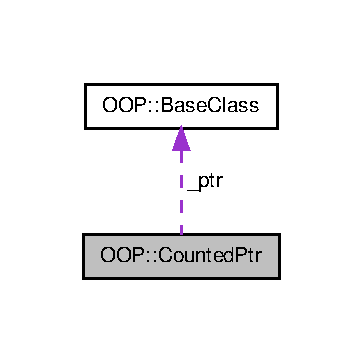
\includegraphics[width=174pt]{classOOP_1_1CountedPtr__coll__graph}
\end{center}
\end{figure}
\subsection*{\-Public \-Member \-Functions}
\begin{DoxyCompactItemize}
\item 
\hyperlink{classOOP_1_1CountedPtr_ae4ac1ddad6538a7281548fd57f5ce158}{\-Counted\-Ptr} ()
\begin{DoxyCompactList}\small\item\em konstruktor domyslny \end{DoxyCompactList}\item 
\hyperlink{classOOP_1_1CountedPtr_a9e67f7da194834072589bca1dce8ccd1}{\-Counted\-Ptr} (\hyperlink{namespaceOOP_a98bf9fa44d8f36499284c9d57c1958aa}{value\-\_\-type} $\ast$)
\item 
\hyperlink{classOOP_1_1CountedPtr_ac5c681d51cd855f36324c467a815618e}{\-Counted\-Ptr} (const \hyperlink{classOOP_1_1CountedPtr}{\-Counted\-Ptr} \&sm)
\item 
\hyperlink{classOOP_1_1CountedPtr}{\-Counted\-Ptr} \& \hyperlink{classOOP_1_1CountedPtr_a36dcaf2d0c344daccdee0a4a51f78728}{operator=} (\hyperlink{classOOP_1_1CountedPtr}{\-Counted\-Ptr} \&sm)
\item 
\hyperlink{classOOP_1_1CountedPtr}{\-Counted\-Ptr} \& \hyperlink{classOOP_1_1CountedPtr_af0a02d043048c2320399f8da522b7d83}{operator=} (\hyperlink{namespaceOOP_a98bf9fa44d8f36499284c9d57c1958aa}{value\-\_\-type} $\ast$)
\item 
\hyperlink{classOOP_1_1CountedPtr_ac4722fd3d5938a1527492acfe4a65a8c}{$\sim$\-Counted\-Ptr} ()
\item 
\hyperlink{namespaceOOP_a98bf9fa44d8f36499284c9d57c1958aa}{value\-\_\-type} $\ast$ \hyperlink{classOOP_1_1CountedPtr_ab2b2a4dc75829686c60fff3194da9cb9}{operator-\/$>$} () const 
\item 
\hyperlink{namespaceOOP_a98bf9fa44d8f36499284c9d57c1958aa}{value\-\_\-type} \& \hyperlink{classOOP_1_1CountedPtr_a2c840594d489eb2f7016e5da227f95e2}{operator$\ast$} () const 
\end{DoxyCompactItemize}
\subsection*{\-Private \-Attributes}
\begin{DoxyCompactItemize}
\item 
\hyperlink{namespaceOOP_a98bf9fa44d8f36499284c9d57c1958aa}{value\-\_\-type} $\ast$ \hyperlink{classOOP_1_1CountedPtr_a2bd5db7ffc59b7811e484c3e858950bd}{\-\_\-ptr}
\item 
int \hyperlink{classOOP_1_1CountedPtr_af164c5e11320b91ea4744fe23c6c3d5b}{\-\_\-licznik}
\end{DoxyCompactItemize}
\subsection*{\-Friends}
\begin{DoxyCompactItemize}
\item 
void \hyperlink{classOOP_1_1CountedPtr_a8a63fdc403051bf98b236855584dbe57}{print\-\_\-tab\-\_\-el} (const \hyperlink{classOOP_1_1array}{array} \&tab2)
\begin{DoxyCompactList}\small\item\em funkcja zaprzyjaźnina \end{DoxyCompactList}\end{DoxyCompactItemize}


\subsection{\-Constructor \& \-Destructor \-Documentation}
\hypertarget{classOOP_1_1CountedPtr_ae4ac1ddad6538a7281548fd57f5ce158}{\index{\-O\-O\-P\-::\-Counted\-Ptr@{\-O\-O\-P\-::\-Counted\-Ptr}!\-Counted\-Ptr@{\-Counted\-Ptr}}
\index{\-Counted\-Ptr@{\-Counted\-Ptr}!OOP::CountedPtr@{\-O\-O\-P\-::\-Counted\-Ptr}}
\subsubsection[{\-Counted\-Ptr}]{\setlength{\rightskip}{0pt plus 5cm}{\bf \-O\-O\-P\-::\-Counted\-Ptr\-::\-Counted\-Ptr} (
\begin{DoxyParamCaption}
{}
\end{DoxyParamCaption}
)\hspace{0.3cm}{\ttfamily  \mbox{[}inline\mbox{]}}}}\label{classOOP_1_1CountedPtr_ae4ac1ddad6538a7281548fd57f5ce158}


konstruktor domyslny 

\hypertarget{classOOP_1_1CountedPtr_a9e67f7da194834072589bca1dce8ccd1}{\index{\-O\-O\-P\-::\-Counted\-Ptr@{\-O\-O\-P\-::\-Counted\-Ptr}!\-Counted\-Ptr@{\-Counted\-Ptr}}
\index{\-Counted\-Ptr@{\-Counted\-Ptr}!OOP::CountedPtr@{\-O\-O\-P\-::\-Counted\-Ptr}}
\subsubsection[{\-Counted\-Ptr}]{\setlength{\rightskip}{0pt plus 5cm}{\bf \-O\-O\-P\-::\-Counted\-Ptr\-::\-Counted\-Ptr} (
\begin{DoxyParamCaption}
\item[{{\bf value\-\_\-type} $\ast$}]{ptr}
\end{DoxyParamCaption}
)}}\label{classOOP_1_1CountedPtr_a9e67f7da194834072589bca1dce8ccd1}
konstruktor konwertujący \hypertarget{classOOP_1_1CountedPtr_ac5c681d51cd855f36324c467a815618e}{\index{\-O\-O\-P\-::\-Counted\-Ptr@{\-O\-O\-P\-::\-Counted\-Ptr}!\-Counted\-Ptr@{\-Counted\-Ptr}}
\index{\-Counted\-Ptr@{\-Counted\-Ptr}!OOP::CountedPtr@{\-O\-O\-P\-::\-Counted\-Ptr}}
\subsubsection[{\-Counted\-Ptr}]{\setlength{\rightskip}{0pt plus 5cm}{\bf \-O\-O\-P\-::\-Counted\-Ptr\-::\-Counted\-Ptr} (
\begin{DoxyParamCaption}
\item[{const {\bf \-Counted\-Ptr} \&}]{sm}
\end{DoxyParamCaption}
)}}\label{classOOP_1_1CountedPtr_ac5c681d51cd855f36324c467a815618e}
konstuktor kopiujący \hypertarget{classOOP_1_1CountedPtr_ac4722fd3d5938a1527492acfe4a65a8c}{\index{\-O\-O\-P\-::\-Counted\-Ptr@{\-O\-O\-P\-::\-Counted\-Ptr}!$\sim$\-Counted\-Ptr@{$\sim$\-Counted\-Ptr}}
\index{$\sim$\-Counted\-Ptr@{$\sim$\-Counted\-Ptr}!OOP::CountedPtr@{\-O\-O\-P\-::\-Counted\-Ptr}}
\subsubsection[{$\sim$\-Counted\-Ptr}]{\setlength{\rightskip}{0pt plus 5cm}{\bf \-O\-O\-P\-::\-Counted\-Ptr\-::$\sim$\-Counted\-Ptr} (
\begin{DoxyParamCaption}
{}
\end{DoxyParamCaption}
)}}\label{classOOP_1_1CountedPtr_ac4722fd3d5938a1527492acfe4a65a8c}


\subsection{\-Member \-Function \-Documentation}
\hypertarget{classOOP_1_1CountedPtr_a2c840594d489eb2f7016e5da227f95e2}{\index{\-O\-O\-P\-::\-Counted\-Ptr@{\-O\-O\-P\-::\-Counted\-Ptr}!operator$\ast$@{operator$\ast$}}
\index{operator$\ast$@{operator$\ast$}!OOP::CountedPtr@{\-O\-O\-P\-::\-Counted\-Ptr}}
\subsubsection[{operator$\ast$}]{\setlength{\rightskip}{0pt plus 5cm}{\bf value\-\_\-type} \& \-O\-O\-P\-::\-Counted\-Ptr\-::operator$\ast$ (
\begin{DoxyParamCaption}
{}
\end{DoxyParamCaption}
) const}}\label{classOOP_1_1CountedPtr_a2c840594d489eb2f7016e5da227f95e2}
przyladowany operator dereferencji \hypertarget{classOOP_1_1CountedPtr_ab2b2a4dc75829686c60fff3194da9cb9}{\index{\-O\-O\-P\-::\-Counted\-Ptr@{\-O\-O\-P\-::\-Counted\-Ptr}!operator-\/$>$@{operator-\/$>$}}
\index{operator-\/$>$@{operator-\/$>$}!OOP::CountedPtr@{\-O\-O\-P\-::\-Counted\-Ptr}}
\subsubsection[{operator-\/$>$}]{\setlength{\rightskip}{0pt plus 5cm}{\bf value\-\_\-type} $\ast$ \-O\-O\-P\-::\-Counted\-Ptr\-::operator-\/$>$ (
\begin{DoxyParamCaption}
{}
\end{DoxyParamCaption}
) const}}\label{classOOP_1_1CountedPtr_ab2b2a4dc75829686c60fff3194da9cb9}
przeładowany operator dostępu \hypertarget{classOOP_1_1CountedPtr_a36dcaf2d0c344daccdee0a4a51f78728}{\index{\-O\-O\-P\-::\-Counted\-Ptr@{\-O\-O\-P\-::\-Counted\-Ptr}!operator=@{operator=}}
\index{operator=@{operator=}!OOP::CountedPtr@{\-O\-O\-P\-::\-Counted\-Ptr}}
\subsubsection[{operator=}]{\setlength{\rightskip}{0pt plus 5cm}{\bf \-Counted\-Ptr} \& \-O\-O\-P\-::\-Counted\-Ptr\-::operator= (
\begin{DoxyParamCaption}
\item[{{\bf \-Counted\-Ptr} \&}]{sm}
\end{DoxyParamCaption}
)}}\label{classOOP_1_1CountedPtr_a36dcaf2d0c344daccdee0a4a51f78728}
operator przypisania 
\begin{DoxyParams}{\-Parameters}
{\em sm} & referencja do zmyślnego wskaźnika \\
\hline
\end{DoxyParams}
\hypertarget{classOOP_1_1CountedPtr_af0a02d043048c2320399f8da522b7d83}{\index{\-O\-O\-P\-::\-Counted\-Ptr@{\-O\-O\-P\-::\-Counted\-Ptr}!operator=@{operator=}}
\index{operator=@{operator=}!OOP::CountedPtr@{\-O\-O\-P\-::\-Counted\-Ptr}}
\subsubsection[{operator=}]{\setlength{\rightskip}{0pt plus 5cm}{\bf \-Counted\-Ptr} \& \-O\-O\-P\-::\-Counted\-Ptr\-::operator= (
\begin{DoxyParamCaption}
\item[{{\bf value\-\_\-type} $\ast$}]{sm}
\end{DoxyParamCaption}
)}}\label{classOOP_1_1CountedPtr_af0a02d043048c2320399f8da522b7d83}
operator przypisania 
\begin{DoxyParams}{\-Parameters}
{\em sm} & referencja do do typu wskazywanego \\
\hline
\end{DoxyParams}


\subsection{\-Friends \-And \-Related \-Function \-Documentation}
\hypertarget{classOOP_1_1CountedPtr_a8a63fdc403051bf98b236855584dbe57}{\index{\-O\-O\-P\-::\-Counted\-Ptr@{\-O\-O\-P\-::\-Counted\-Ptr}!print\-\_\-tab\-\_\-el@{print\-\_\-tab\-\_\-el}}
\index{print\-\_\-tab\-\_\-el@{print\-\_\-tab\-\_\-el}!OOP::CountedPtr@{\-O\-O\-P\-::\-Counted\-Ptr}}
\subsubsection[{print\-\_\-tab\-\_\-el}]{\setlength{\rightskip}{0pt plus 5cm}void {\bf print\-\_\-tab\-\_\-el} (
\begin{DoxyParamCaption}
\item[{const {\bf array} \&}]{tab2}
\end{DoxyParamCaption}
)\hspace{0.3cm}{\ttfamily  \mbox{[}friend\mbox{]}}}}\label{classOOP_1_1CountedPtr_a8a63fdc403051bf98b236855584dbe57}


funkcja zaprzyjaźnina 

/param tab2 referencja do elemnetu tablicy 

\subsection{\-Member \-Data \-Documentation}
\hypertarget{classOOP_1_1CountedPtr_af164c5e11320b91ea4744fe23c6c3d5b}{\index{\-O\-O\-P\-::\-Counted\-Ptr@{\-O\-O\-P\-::\-Counted\-Ptr}!\-\_\-licznik@{\-\_\-licznik}}
\index{\-\_\-licznik@{\-\_\-licznik}!OOP::CountedPtr@{\-O\-O\-P\-::\-Counted\-Ptr}}
\subsubsection[{\-\_\-licznik}]{\setlength{\rightskip}{0pt plus 5cm}int {\bf \-O\-O\-P\-::\-Counted\-Ptr\-::\-\_\-licznik}\hspace{0.3cm}{\ttfamily  \mbox{[}private\mbox{]}}}}\label{classOOP_1_1CountedPtr_af164c5e11320b91ea4744fe23c6c3d5b}
\hypertarget{classOOP_1_1CountedPtr_a2bd5db7ffc59b7811e484c3e858950bd}{\index{\-O\-O\-P\-::\-Counted\-Ptr@{\-O\-O\-P\-::\-Counted\-Ptr}!\-\_\-ptr@{\-\_\-ptr}}
\index{\-\_\-ptr@{\-\_\-ptr}!OOP::CountedPtr@{\-O\-O\-P\-::\-Counted\-Ptr}}
\subsubsection[{\-\_\-ptr}]{\setlength{\rightskip}{0pt plus 5cm}{\bf value\-\_\-type}$\ast$ {\bf \-O\-O\-P\-::\-Counted\-Ptr\-::\-\_\-ptr}\hspace{0.3cm}{\ttfamily  \mbox{[}private\mbox{]}}}}\label{classOOP_1_1CountedPtr_a2bd5db7ffc59b7811e484c3e858950bd}
wskaznik na pokazywany typ 

\-The documentation for this class was generated from the following files\-:\begin{DoxyCompactItemize}
\item 
\hyperlink{CountedPtr_8h}{\-Counted\-Ptr.\-h}\item 
\hyperlink{CountedPtr_8cpp}{\-Counted\-Ptr.\-cpp}\end{DoxyCompactItemize}

\chapter{\-File \-Documentation}
\hypertarget{array_8cpp}{\section{array.\-cpp \-File \-Reference}
\label{array_8cpp}\index{array.\-cpp@{array.\-cpp}}
}
{\ttfamily \#include \char`\"{}\-Counted\-Ptr.\-h\char`\"{}}\*
{\ttfamily \#include \char`\"{}array.\-h\char`\"{}}\*
\-Include dependency graph for array.\-cpp\-:
\nopagebreak
\begin{figure}[H]
\begin{center}
\leavevmode
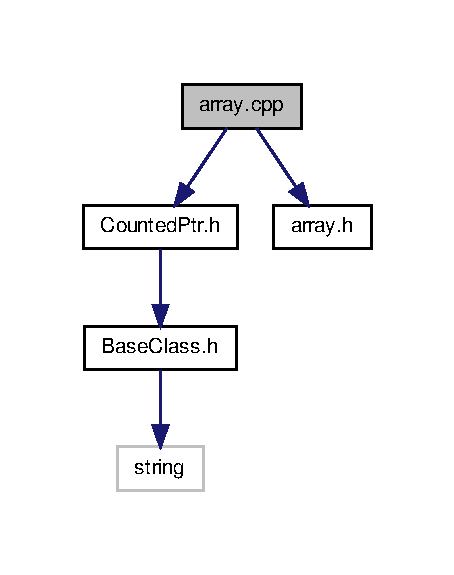
\includegraphics[width=218pt]{array_8cpp__incl}
\end{center}
\end{figure}
\subsection*{\-Namespaces}
\begin{DoxyCompactItemize}
\item 
namespace \hyperlink{namespaceOOP}{\-O\-O\-P}
\end{DoxyCompactItemize}

\hypertarget{array_8h}{\section{array.\-h \-File \-Reference}
\label{array_8h}\index{array.\-h@{array.\-h}}
}
\-This graph shows which files directly or indirectly include this file\-:\nopagebreak
\begin{figure}[H]
\begin{center}
\leavevmode
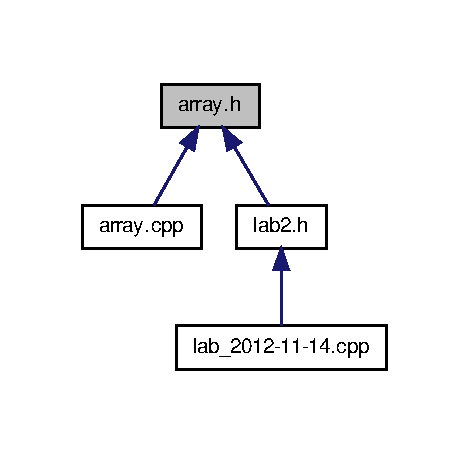
\includegraphics[width=225pt]{array_8h__dep__incl}
\end{center}
\end{figure}
\subsection*{\-Classes}
\begin{DoxyCompactItemize}
\item 
class \hyperlink{classOOP_1_1array}{\-O\-O\-P\-::array}
\end{DoxyCompactItemize}
\subsection*{\-Namespaces}
\begin{DoxyCompactItemize}
\item 
namespace \hyperlink{namespaceOOP}{\-O\-O\-P}
\begin{DoxyCompactList}\small\item\em plik zawiera klase counted \-Ptr \end{DoxyCompactList}\end{DoxyCompactItemize}

\hypertarget{BaseClass_8cpp}{\section{\-Base\-Class.\-cpp \-File \-Reference}
\label{BaseClass_8cpp}\index{\-Base\-Class.\-cpp@{\-Base\-Class.\-cpp}}
}
{\ttfamily \#include \char`\"{}\-Base\-Class.\-h\char`\"{}}\*
\-Include dependency graph for \-Base\-Class.\-cpp\-:\nopagebreak
\begin{figure}[H]
\begin{center}
\leavevmode
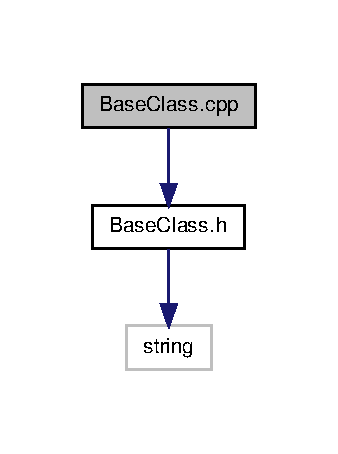
\includegraphics[width=162pt]{BaseClass_8cpp__incl}
\end{center}
\end{figure}
\subsection*{\-Namespaces}
\begin{DoxyCompactItemize}
\item 
namespace \hyperlink{namespaceOOP}{\-O\-O\-P}
\begin{DoxyCompactList}\small\item\em plik zawiera klase counted \-Ptr \end{DoxyCompactList}\end{DoxyCompactItemize}

\hypertarget{BaseClass_8h}{\section{\-Base\-Class.\-h \-File \-Reference}
\label{BaseClass_8h}\index{\-Base\-Class.\-h@{\-Base\-Class.\-h}}
}
{\ttfamily \#include $<$string$>$}\*
\-Include dependency graph for \-Base\-Class.\-h\-:\nopagebreak
\begin{figure}[H]
\begin{center}
\leavevmode
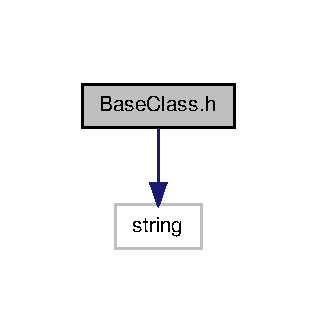
\includegraphics[width=152pt]{BaseClass_8h__incl}
\end{center}
\end{figure}
\-This graph shows which files directly or indirectly include this file\-:\nopagebreak
\begin{figure}[H]
\begin{center}
\leavevmode
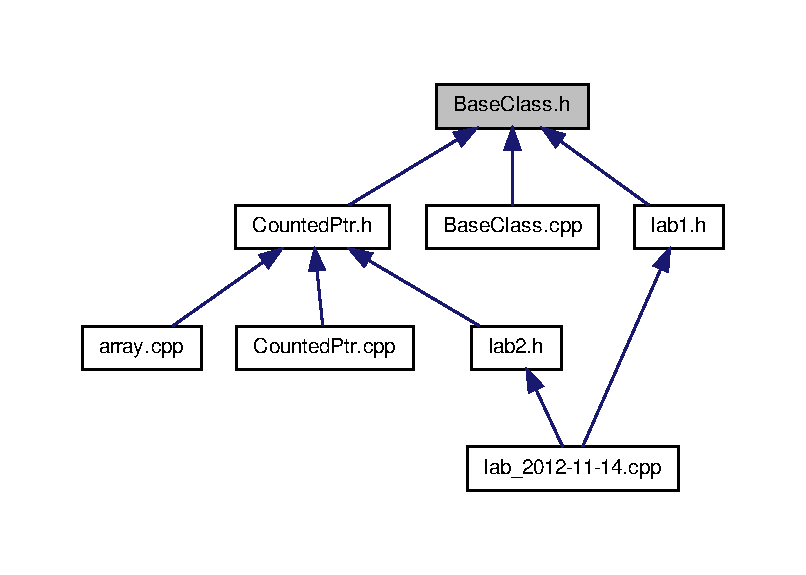
\includegraphics[width=350pt]{BaseClass_8h__dep__incl}
\end{center}
\end{figure}
\subsection*{\-Classes}
\begin{DoxyCompactItemize}
\item 
class \hyperlink{classOOP_1_1BaseClass}{\-O\-O\-P\-::\-Base\-Class}
\end{DoxyCompactItemize}
\subsection*{\-Namespaces}
\begin{DoxyCompactItemize}
\item 
namespace \hyperlink{namespaceOOP}{\-O\-O\-P}
\begin{DoxyCompactList}\small\item\em plik zawiera klase counted \-Ptr \end{DoxyCompactList}\end{DoxyCompactItemize}

\hypertarget{CountedPtr_8cpp}{\section{\-Counted\-Ptr.\-cpp \-File \-Reference}
\label{CountedPtr_8cpp}\index{\-Counted\-Ptr.\-cpp@{\-Counted\-Ptr.\-cpp}}
}
{\ttfamily \#include \char`\"{}\-Counted\-Ptr.\-h\char`\"{}}\*
\-Include dependency graph for \-Counted\-Ptr.\-cpp\-:
\nopagebreak
\begin{figure}[H]
\begin{center}
\leavevmode
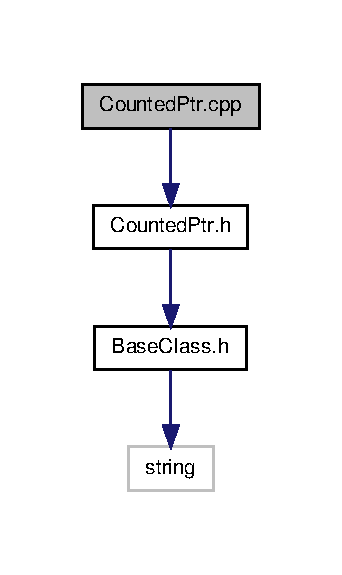
\includegraphics[width=164pt]{CountedPtr_8cpp__incl}
\end{center}
\end{figure}
\subsection*{\-Namespaces}
\begin{DoxyCompactItemize}
\item 
namespace \hyperlink{namespaceOOP}{\-O\-O\-P}
\end{DoxyCompactItemize}

\hypertarget{CountedPtr_8h}{\section{src/\-Counted\-Ptr.h \-File \-Reference}
\label{CountedPtr_8h}\index{src/\-Counted\-Ptr.\-h@{src/\-Counted\-Ptr.\-h}}
}
\subsection*{\-Classes}
\begin{DoxyCompactItemize}
\item 
class \hyperlink{classCountedPtr}{\-Counted\-Ptr}
\end{DoxyCompactItemize}
\subsection*{\-Defines}
\begin{DoxyCompactItemize}
\item 
\#define \hyperlink{CountedPtr_8h_a26a95ee06b3c1c2d31618cc2d1fc49e8}{\-I\-N\-T\-\_\-\-B\-A\-S\-E\-D\-\_\-\-P\-T\-R}
\end{DoxyCompactItemize}
\subsection*{\-Typedefs}
\begin{DoxyCompactItemize}
\item 
typedef \hyperlink{classInt__t}{\-Int\-\_\-t} \hyperlink{CountedPtr_8h_a29b8e20df76c705cc065fde787679528}{value\-\_\-type}
\end{DoxyCompactItemize}


\subsection{\-Define \-Documentation}
\hypertarget{CountedPtr_8h_a26a95ee06b3c1c2d31618cc2d1fc49e8}{\index{\-Counted\-Ptr.\-h@{\-Counted\-Ptr.\-h}!\-I\-N\-T\-\_\-\-B\-A\-S\-E\-D\-\_\-\-P\-T\-R@{\-I\-N\-T\-\_\-\-B\-A\-S\-E\-D\-\_\-\-P\-T\-R}}
\index{\-I\-N\-T\-\_\-\-B\-A\-S\-E\-D\-\_\-\-P\-T\-R@{\-I\-N\-T\-\_\-\-B\-A\-S\-E\-D\-\_\-\-P\-T\-R}!CountedPtr.h@{\-Counted\-Ptr.\-h}}
\subsubsection[{\-I\-N\-T\-\_\-\-B\-A\-S\-E\-D\-\_\-\-P\-T\-R}]{\setlength{\rightskip}{0pt plus 5cm}\#define {\bf \-I\-N\-T\-\_\-\-B\-A\-S\-E\-D\-\_\-\-P\-T\-R}}}\label{CountedPtr_8h_a26a95ee06b3c1c2d31618cc2d1fc49e8}


\subsection{\-Typedef \-Documentation}
\hypertarget{CountedPtr_8h_a29b8e20df76c705cc065fde787679528}{\index{\-Counted\-Ptr.\-h@{\-Counted\-Ptr.\-h}!value\-\_\-type@{value\-\_\-type}}
\index{value\-\_\-type@{value\-\_\-type}!CountedPtr.h@{\-Counted\-Ptr.\-h}}
\subsubsection[{value\-\_\-type}]{\setlength{\rightskip}{0pt plus 5cm}typedef {\bf \-Int\-\_\-t} {\bf value\-\_\-type}}}\label{CountedPtr_8h_a29b8e20df76c705cc065fde787679528}

\hypertarget{lab1_8h}{\section{lab1.\-h \-File \-Reference}
\label{lab1_8h}\index{lab1.\-h@{lab1.\-h}}
}
{\ttfamily \#include \char`\"{}\-Base\-Class.\-h\char`\"{}}\*
{\ttfamily \#include $<$stdlib.\-h$>$}\*
\-Include dependency graph for lab1.\-h\-:\nopagebreak
\begin{figure}[H]
\begin{center}
\leavevmode
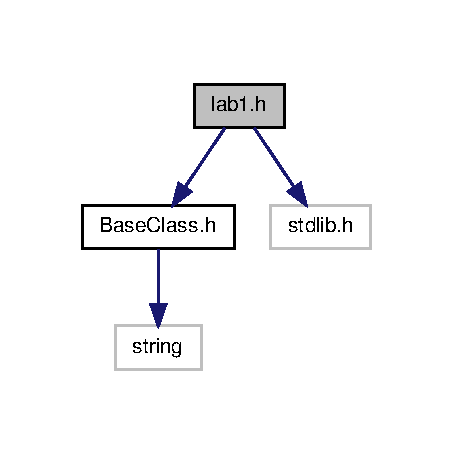
\includegraphics[width=218pt]{lab1_8h__incl}
\end{center}
\end{figure}
\-This graph shows which files directly or indirectly include this file\-:\nopagebreak
\begin{figure}[H]
\begin{center}
\leavevmode
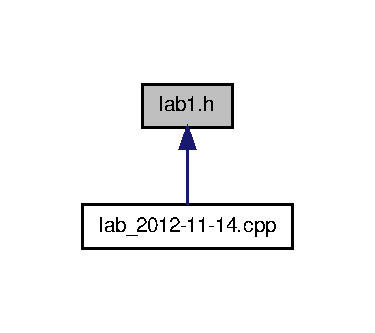
\includegraphics[width=180pt]{lab1_8h__dep__incl}
\end{center}
\end{figure}

\hypertarget{lab2_8h}{\section{lab2.\-h \-File \-Reference}
\label{lab2_8h}\index{lab2.\-h@{lab2.\-h}}
}
{\ttfamily \#include $<$iostream$>$}\*
{\ttfamily \#include \char`\"{}\-Counted\-Ptr.\-h\char`\"{}}\*
{\ttfamily \#include \char`\"{}array.\-h\char`\"{}}\*
\-Include dependency graph for lab2.\-h\-:\nopagebreak
\begin{figure}[H]
\begin{center}
\leavevmode
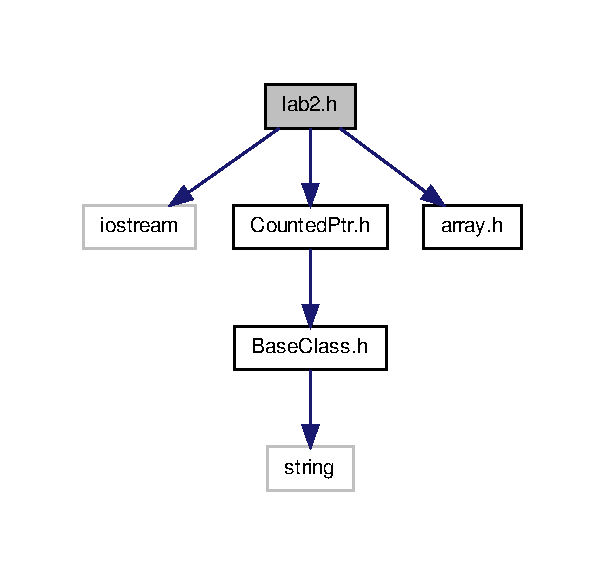
\includegraphics[width=290pt]{lab2_8h__incl}
\end{center}
\end{figure}
\-This graph shows which files directly or indirectly include this file\-:\nopagebreak
\begin{figure}[H]
\begin{center}
\leavevmode
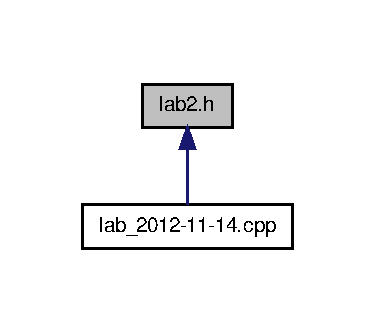
\includegraphics[width=180pt]{lab2_8h__dep__incl}
\end{center}
\end{figure}
\subsection*{\-Namespaces}
\begin{DoxyCompactItemize}
\item 
namespace \hyperlink{namespaceOOP}{\-O\-O\-P}
\begin{DoxyCompactList}\small\item\em plik zawiera klase counted \-Ptr \end{DoxyCompactList}\end{DoxyCompactItemize}
\subsection*{\-Functions}
\begin{DoxyCompactItemize}
\item 
void \hyperlink{namespaceOOP_a32e75bb4328dbb5e86e98a8af0a5cf61}{\-O\-O\-P\-::print\-\_\-tab\-\_\-el} (const array \&tab2)
\item 
ostream \& \hyperlink{namespaceOOP_a3f50dd68985954d3519768fe0da14797}{\-O\-O\-P\-::operator$<$$<$} (ostream \&stream, \-Base\-Class \&base)
\end{DoxyCompactItemize}

\hypertarget{lab__2012-11-14_8cpp}{\section{lab\-\_\-2012-\/11-\/14.cpp \-File \-Reference}
\label{lab__2012-11-14_8cpp}\index{lab\-\_\-2012-\/11-\/14.\-cpp@{lab\-\_\-2012-\/11-\/14.\-cpp}}
}
{\ttfamily \#include \char`\"{}lab1.\-h\char`\"{}}\*
{\ttfamily \#include \char`\"{}lab2.\-h\char`\"{}}\*
{\ttfamily \#include $<$stdlib.\-h$>$}\*
\-Include dependency graph for lab\-\_\-2012-\/11-\/14.cpp\-:\nopagebreak
\begin{figure}[H]
\begin{center}
\leavevmode
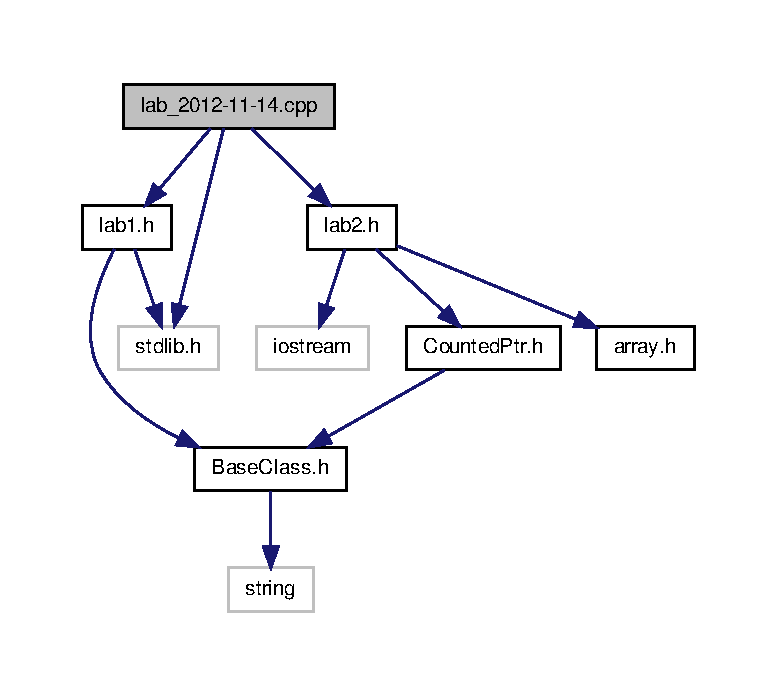
\includegraphics[width=350pt]{lab__2012-11-14_8cpp__incl}
\end{center}
\end{figure}
\subsection*{\-Typedefs}
\begin{DoxyCompactItemize}
\item 
typedef \hyperlink{classOOP_1_1BaseClass}{\-O\-O\-P\-::\-Base\-Class} \hyperlink{lab__2012-11-14_8cpp_a1ebf4c1886eac7249b0dce3557d4a720}{value\-\_\-type}
\end{DoxyCompactItemize}
\subsection*{\-Functions}
\begin{DoxyCompactItemize}
\item 
int \hyperlink{lab__2012-11-14_8cpp_ae66f6b31b5ad750f1fe042a706a4e3d4}{main} ()
\end{DoxyCompactItemize}


\subsection{\-Typedef \-Documentation}
\hypertarget{lab__2012-11-14_8cpp_a1ebf4c1886eac7249b0dce3557d4a720}{\index{lab\-\_\-2012-\/11-\/14.\-cpp@{lab\-\_\-2012-\/11-\/14.\-cpp}!value\-\_\-type@{value\-\_\-type}}
\index{value\-\_\-type@{value\-\_\-type}!lab_2012-11-14.cpp@{lab\-\_\-2012-\/11-\/14.\-cpp}}
\subsubsection[{value\-\_\-type}]{\setlength{\rightskip}{0pt plus 5cm}typedef {\bf \-O\-O\-P\-::\-Base\-Class} {\bf value\-\_\-type}}}\label{lab__2012-11-14_8cpp_a1ebf4c1886eac7249b0dce3557d4a720}


\subsection{\-Function \-Documentation}
\hypertarget{lab__2012-11-14_8cpp_ae66f6b31b5ad750f1fe042a706a4e3d4}{\index{lab\-\_\-2012-\/11-\/14.\-cpp@{lab\-\_\-2012-\/11-\/14.\-cpp}!main@{main}}
\index{main@{main}!lab_2012-11-14.cpp@{lab\-\_\-2012-\/11-\/14.\-cpp}}
\subsubsection[{main}]{\setlength{\rightskip}{0pt plus 5cm}int {\bf main} (
\begin{DoxyParamCaption}
{}
\end{DoxyParamCaption}
)}}\label{lab__2012-11-14_8cpp_ae66f6b31b5ad750f1fe042a706a4e3d4}

\printindex
\end{document}
